\section{Resolución de Problemas}
\begin{enumerate}
    \item
    Implemente los siguientes algoritmos de ordenación. Si no está familiarizado con alguno de ellos, consulte alguna fuente confiable para estudiar su funcionamiento:
\begin{enumerate}
    \item Ordenación por Burbuja (Bubble Sort)
    \item Ordenación por Mínimos Sucesivos (Selection Sort)
    \item Ordenación por Inserción (Insertion Sort)
    \item Ordenación por Conteo, para arrays de enteros no negativos (Counting Sort)
\end{enumerate}

    \item 
    Escriba un método que dado un array de números enteros devuelva la menor de las diferencias entre cualquier par de elementos.

\subsection*{Ejemplos}

\begin{itemize}
    \item Si el arreglo es \([4, 9, 1, 32, 13, 6]\), la menor diferencia entre cualquier par de elementos es \(2\), la diferencia entre \(4\) y \(6\)).
    \item Si el arreglo es \([10, 20, 30, 40]\), la menor diferencia es \(10\).
    \item Si el arreglo es \([5, 5, 5]\), la menor diferencia es \(0\).
\end{itemize}

\textbf{Aclaración:} El arreglo debe contener al menos dos elementos.


    \item 
    Sea \( a \) un array de enteros y \( k \) un entero positivo. Implemente un método que determine si en \( a \) existen \( k \) elementos consecutivos iguales.

\subsection*{Ejemplos}

\begin{itemize}
    \item Para \( a = [1, 2, 2, 2, 3, 4] \) y \( k = 3 \), la salida debe ser \textcolor{blue}{true}, ya que \( 2 \) aparece tres veces consecutivas.
    \item Para \( a = [5, 5, 6, 6, 6, 7] \) y \( k = 4 \), la salida debe ser \textcolor{blue}{false}, ya que no hay ningún número que aparezca cuatro veces consecutivas.
    \item Para \( a = [1, 1, 1, 1, 1] \) y \( k = 5 \), la salida debe ser \textcolor{blue}{true}, ya que \( 1 \) aparece cinco veces consecutivas.
\end{itemize}

    \item
    Implemente un método que devuelva los elementos de un array de enteros por orden de cercanía a otro entero dado que llamaremos \texttt{pivote}. En caso de que existan varios elementos en el array a la misma distancia del elemento pivote, estos se deberán ordenar de menor a mayor entre ellos.

\subsection*{Ejemplos}

\begin{itemize}
    \item Para el array \([5, 3, 7, 10]\) y \texttt{pivote} = 7, los elementos del array quedarían: 
    \[
    [7,5,10,3]
    \]
    
    \item Para el array \([4, 2, 11, 8]\) y \texttt{pivote} = 7, los elementos del array quedarían:
    \[
    [8, 4, 11, 2]
    \]
    Note que el elemento pivote puede o no pertenecer al array.

    \item Para el array \([2, 10, 8, 4]\) y \texttt{pivote} = 7, los elementos del array quedarían:
    \[
    [8, 4, 10, 2]
    \]
    Note que los elementos 4 y 10 están a la misma distancia del pivote. En este caso, el orden correcto es que 4 aparezca antes de 10, ya que es menor.
\end{itemize}

    \item 
    Implemente un método que dado un array de números enteros, devuelva la suma del subarray de suma máxima. Si todos los números son negativos devolver 0.

\subsection*{Ejemplos}

\begin{itemize}
    \item Para el arreglo \([1, 1, -3, 4, 2, 2, -1, 2, -3, 2]\):
    \begin{itemize}
        \item El subarray de suma máxima es \([1, 1, -3, \textcolor{green}{4}, \textcolor{green}{2}, \textcolor{green}{2}, \textcolor{green}{-1}, \textcolor{green}{2}, -3, 2]\).
        \item La suma es \(4 + 2 + 2 - 1 + 2 = 9\).
    \end{itemize}
    Resultado: \(9\).
    
    \item Para el arreglo \([-4, -2, -7, -1]\):
    \begin{itemize}
        \item Todos los números son negativos, por lo que no existe un subarray positivo.
        \item El resultado es \(0\), representando un subarray vacío.
    \end{itemize}
    Resultado: \(0\).
    
    \item Para el arreglo \([3, -2, 5, -1, 6, -3, 2]\):
    \begin{itemize}
        \item El subarray de suma máxima es \([\textcolor{green}{3}, \textcolor{green}{-2}, \textcolor{green}{5}, \textcolor{green}{-1}, \textcolor{green}{6}, -3, 2]\).
        \item La suma es \(3 - 2 + 5 - 1 + 6 = 11\).
    \end{itemize}
    Resultado: \(11\).

    \item Para el arreglo \([0, -1, 0, -2, 0, -3]\):
    \begin{itemize}
        \item Todos los números son negativos o ceros, por lo que no existe un subarray con suma positiva. Un subarray de suma máxima sería \([\textcolor{green}{0}, -1, 0, -2, 0, -3]\)
    \end{itemize}
    Resultado: \(0\).
\end{itemize}


    \item 
    Un anagrama de una palabra es cualquier otra palabra que tenga las mismas letras que la primera pero en distinto orden.

\begin{enumerate}
    \item Implemente un método que dadas dos palabras determine si son un anagrama.

    \subsection*{Ejemplos}
    \begin{itemize}
    \item \texttt{casa} y \texttt{saca}.
    \item \texttt{tasa} y \texttt{asta}.
    \end{itemize}

    \item Implemente un método que dado un grupo de palabras (string[]) devuelva la cantidad de palabras del mayor subconjunto de anagramas que se pueda formar.

    Dado el arreglo de entrada:
    \[
    \texttt{[''amor'', ''cometa'', ''roma'', ''mora'', ''moceta'']}
    \]
    El mayor subconjunto de anagramas contiene las palabras:
    \[
    \texttt{''amor'', ''roma'', ''mora''}
    \]
    Por lo tanto, el método debe devolver: \( \texttt{3} \)
\end{enumerate}

    \item
    Implemente un método que dado un texto, devuelva el número de ocurrencias de una palabra en él.

\subsection*{Ejemplos}

\begin{itemize}
    \item Para el texto: \texttt{''El agua es muy importante para la vida, entre otras razones porque con ella riegan las plantas.''}  
    y la palabra: \texttt{''agua''}, el resultado es \(1\).

    \item Para el texto: \texttt{''anana''}  
    y la palabra: \texttt{''ana''}, el resultado es \(2\).

    \item Para el texto: \texttt{''abcabcabc''}  
    y la palabra: \texttt{''abc''}, el resultado es \(3\).

    \item Para el texto: \texttt{''mississippi''}  
    y la palabra: \texttt{''issi''}, el resultado es \(2\). 
\end{itemize}

\textbf{Nota:} El método debe considerar las ocurrencias superpuestas. Por ejemplo, en el texto \texttt{anana} la palabra \texttt{''ana''} aparece dos veces:  
\[
\texttt{anana} \quad \rightarrow \quad \texttt{\underline{ana}na}, \quad \texttt{a\underline{ana}}.
\]


    \item
    Escriba un método que dado un entero \(n\) devuelva un array de bool de tamaño \(n\), donde la posición \(i\) tendrá valor \textcolor{blue}{true} si el número entero \(i\) es primo, en caso contrario, tendrá valor  \textcolor{blue}{false}. 


    \item
    Implemente un método que reciba un entero \(k\) y un array de valores y devuelva cuántos de esos valores se repiten exactamente \(k\) veces.

\subsection*{Ejemplos}
\begin{itemize}
    \item Entrada: \( k = 2 \), \( arr = [4, 2, 4, 5, 6, 2, 7] \) \\
          Salida: \( 2 \) \\
          Explicación: Los números \( 4 \) y \( 2 \) aparecen exactamente \( 2 \) veces.

    \item Entrada: \( k = 3 \), \( arr = [8, 1, 8, 8, 9, 2, 1, 1] \)\\
          Salida: \( 2 \)\\
          Explicación:  Los números \( 8 \) y \( 1 \) aparecen exactamente \( 3 \) veces.

    \item Entrada: \( k = 4 \), \( arr = [7, 7, 7, 7, 8, 9, 10, 8]\)\\
          Salida: \( 1 \) \\
          Explicación: El número \( 7 \) aparece exactamente \( 4 \) veces.

    \item Entrada: \( k = 1 \), \( arr = [3, 5, 3, 5, 7, 7, 7] \) \\
          Salida: \( 0 \)\\
          Explicación: Ningún número aparece exactamente \( 1 \) vez.
\end{itemize}

    \item
    Dado un número entero \( k \) y un arreglo \( arr \) de números distintos, determina cuántos pares \((a, b)\) existen en \( arr \) tales que \( a + b = k \).

\subsection*{Ejemplos}
\begin{itemize}
    \item Entrada: \( k = 5 \), \( arr = [1, 2, 3, 4] \) \\
          Salida: \( 2 \)\\
          Explicación: Los pares que suman \( 5 \) son: \( (1, 4), (2, 3) \).

    \item Entrada: \( k = 8 \), \( arr = [10, 15, 3, 7] \) \\
          Salida: \( 0 \)\\
          Explicación: Ningún par de números suma \( 8 \).

    \item Entrada: \( k = 13 \), \( arr = [5, 7, 1, 6, 11] \) \\
          Salida: \( 1 \)\\
          Explicación: El único par que suma \( 13 \) es: \( (7, 6) \).

    \item Entrada: \( k = 10 \), \( arr = [1, 2, 3, 4, 5, 6, 7, 8, 9] \) \\
          Salida: \( 4 \)\\
          Explicación: Los pares que suman \( 10 \) son: \( (1, 9), (2, 8), (3, 7), (4, 6) \).


    \item Entrada: \( k = 4 \), \( arr = [0, 6, 4, -2, -4] \) \\
          Salida: \( 2 \)\\
          Explicación: Los pares que suman \( 4 \) son: \( (0, 4), (6, -2) \).
\end{itemize}

    \item
    Implemente un método que dado un string s y un string p, devuelva una 
cadena equivalente a quitar de la s la primera subcadena que sea igual a la cadena p. 

Es decir si se invoca con $s = "abracadabra"$ y $"p = cad"$ se debe obtener como resultado la cadena $"abraabra"$.

Si se llama $"s = locoloco"$y $ "p = co"$ debe dar como resultado $"loloco"$


    \item
    Dado un array de \(N\) valores donde cada valor representa la cantidad de chocolates en un paquete, se quieren repartir estos paquetes entre varios estudiantes. Determine cómo distribuirlos de forma tal que se satisfagan las siguientes condiciones:
\begin{itemize}
    \item Cada estudiante recibe exactamente un paquete.
    \item La diferencia entre la cantidad de chocolates del estudiante con la mínima cantidad y la del estudiante con la máxima cantidad es mínima.
\end{itemize}

    \item
    Dado un arreglo \( arr \) de \( n \) elementos, encuentra el número total de \textit{inversiones}. Una inversión se define como un par de índices \( (i, j) \) tal que:

\[
i < j \quad \text{y} \quad arr[i] > arr[j].
\]

\subsection*{Ejemplos}
\begin{itemize}
    \item Entrada: \( arr = [2, 4, 1, 3, 5] \) \\
     Salida: \( 3 \)\\
     Explicación:  Las inversiones son:
    \(
    (2, 1), (4, 1), (4, 3)
    \)

    \item Entrada: \( arr = [5, 4, 3, 2, 1] \) \\
    Salida: \( 10 \)\\
    Explicación:  Todas las parejas \( (i, j) \) con \( i < j \) son inversiones, ya que el arreglo está completamente desordenado.

    \item Entrada: \( arr = [1, 2, 3, 4, 5] \) \\
    Salida: \( 0 \)\\
    Explicación:  El arreglo está completamente ordenado, por lo que no hay inversiones.
\end{itemize}

    
    \item 
    Implemente un método que logre convertir el número $n$ (representado como \textcolor{blue}{string}) que está en la base \texttt{old\_base} a la base \texttt{new\_base}. Tenga en cuenta que ambos (\texttt{old\_base} y \texttt{new\_base}) estarán entre 2 y 36.

    \item
    Un sistema de numeración está definido por una secuencia ordenada de símbolos a los cuales se les asocia valores. Por ejemplo, el sistema decimal (de base diez) que más comúnmente utilizamos está constituido por diez símbolos '0', '1', '2', '3', '4', '5', '6', '7', '8', y '9', que corresponden en este caso a los valores enteros 0, 1, 2, 3, 4, 5, 6, 7, 8, y 9 respectivamente. En este sistema, la secuencia ''475'' expresa el número cuatrocientos setenta y cinco, que es el resultado de:

\[
4 \times 10^2 + 7 \times 10^1 + 5 \times 10^0
\]

Si el sistema estuviese constituido por los tres símbolos 'a', 'b', 'c' (que se asocian a los valores enteros 0, 1 y 2 respectivamente), entonces la secuencia "baac" denotaría al número cuyo valor es \( 1 \times 3^3 + 0 \times 3^2 + 0 \times 3^1 + 2 \times 3^0 \), es decir, 29 en el sistema decimal.

\begin{enumerate}[label=\alph*)]
    \item Implemente un método que, a partir de una secuencia expresada por el string \texttt{numero} representada en una base que es la cantidad de caracteres en el array \texttt{digitosBase}, devuelve el valor de tipo \texttt{int} correspondiente a ese número según la base.

    \textbf{Ejemplo:}
    Para \texttt{numero} = $"baac"$ en la base \texttt{digitosBase} = $['a', 'b', 'c']$ debería devolver 29.

    \item Recíprocamente, implemente un método que devuelva un \texttt{string} que contenga la secuencia de caracteres que representa un número entero en la base dada por el conjunto de caracteres especificado por el parámetro \texttt{digitosBase}.

    \textbf{Ejemplo:}
    Para \texttt{numero} = $29$ en la base \texttt{digitosBase} = $['a', 'b', 'c']$ debería devolver $"baac"$.
\end{enumerate}
\end{enumerate}

\newpage
\section{Array bidimensionales}
\begin{enumerate}
    \item \textbf{Traza de una matriz:}\\
    Implemente un método que reciba una matriz cuadrada (un array bidimensional de tipo entero que representa una matriz algebraica) y devuelva la suma de los elementos de su diagonal.

    \item \textbf{Chequear simetría:}\\
    Implemente un método que reciba una matriz (un array bidimensional de tipo entero que representa una matriz algebraica) y devuelva \textcolor{blue}{true} si es simétrica, \textcolor{blue}{false} en caso contrario.

    \item \textbf{Cuadrado mágico}\\
    Determine si una matriz cuadrada de enteros constituye un cuadrado mágico. Esto es que la suma de todas las filas, las columnas y ambas diagonales sea la misma.


    \item \textbf{Suma de matrices:}\\
    Implemente un método que reciba dos matrices (arrays bidimensionales de tipo entero que representan matrices algebraicas) y devuelva su suma.

    \item \textbf{Transpuesta:}\\
    Implemente un método que reciba una matriz (un array bidimensional de tipo entero que representa una matriz algebraica) y devuelva su transpuesta (intercambiar filas y columnas).

    \item \textbf{Construcción de aeropuertos}\\
    En un terreno de NxM expresado por la cantidad de filas y columnas de una matriz en metros se quiere construir un aeropuerto con área rectangular de Alto x Ancho (que debe caber dentro de la matríz anterior). En cada celda de la matriz se tiene la altura del terreno en ese lugar. El aeropuerto se quiere construir en la zona más "pareja" del terreno, es decir, que teniendo el área requerida en cuanto a cantidad de celdas por la horizontal y por la vertical la diferencia entre la máxima altura y la mínima altura sea la menor.

\textbf{Ejemplo:} La figura a continuación nos muestra en el rectángulo indicado en verde el área adecuada para una pista que tenga que ser de \(3 \times 2\). El rectángulo en rojo nos indica un área que es menos pareja.

\begin{center}
    \begin{tabular}{|l|l|l|l|l|l|}
    \hline
    \cellcolor{blue!20} 4 & \cellcolor{blue!20} 3 & \cellcolor{blue!20} 5 & \cellcolor{blue!20} 1 & \cellcolor{blue!20} 2 & \cellcolor{blue!20} 1 \\
    \hline
    \cellcolor{red!20} 2 & \cellcolor{red!20} 7 & \cellcolor{blue!20} 6 & \cellcolor{blue!20} 3 & \cellcolor{green!20} 2 & \cellcolor{green!20} 3 \\
    \hline
    \cellcolor{red!20} 3 & \cellcolor{red!20} 8 & \cellcolor{blue!20} 5 & \cellcolor{blue!20} 2 & \cellcolor{green!20} 2 & \cellcolor{green!20} 3 \\
    \hline
    \cellcolor{red!20} 5 & \cellcolor{red!20} 7 & \cellcolor{blue!20} 6 & \cellcolor{blue!20} 4 & \cellcolor{green!20} 2 & \cellcolor{green!20} 3 \\
    \hline
    \end{tabular}
\end{center}

\begin{enumerate}[label=\alph*)]
    \item Implemente un método que devuelva la mínima diferencia de alturas de un terreno válido para construir el aeropuerto.
    
    Note que en el área encerrada en verde la diferencia de alturas es \(1\) y en la otra es \(6\), de modo que si se invoca con \(3\) de alto y \(2\) de ancho, debe devolver como resultado \(1.\)
    
    \item * Haga una variante del método anterior pero que devuelva en lugar de la diferencia entre las alturas, las coordenadas del terreno adecuado dadas por la posición fila y columna de la celda esquina superior izquierda del terreno y la fila y columna de la celda esquina inferior derecha del terreno. 
    
    En este caso para la invocación del ejemplo anterior debe devolver el array: \(\{1,4,3,5\}\).
\end{enumerate}

    \item \textbf{Triángulo de Pascal}\\
    Dado un entero \( n \), se quiere construir una matriz de enteros que represente el Triángulo de Pascal hasta el nivel \( n \):
$$
{n\choose k} = {n-1\choose k-1} + {n-1\choose k}
$$
\textbf{Ejemplo:} 

Para \( n = 4\):
\[
\begin{array}{ccccccccc}
    &  &   &   & 1 &   &   \\
    &  &   & 1 &   & 1 &   \\
    &  & 1 &   & 2 &   & 1 \\
    &  1 &  & 3 &   & \textcolor{red}{3} &  & \textcolor{red}{1} \\
  1 & & 4 & & 6 & & \textcolor{green}{4} & & 1 
\end{array}
\]
Quedaría representado por la matriz:
\[
\begin{bmatrix}
    1 & 0 & 0 & 0 & 0 \\
    1 & 1 & 0 & 0 & 0 \\
    1 & 2 & 1 & 0 & 0 \\
    1 & 3 & \textcolor{red}{3} & \textcolor{red}{1} & 0 \\
    1 & 4 & 6 & \textcolor{green}{4} & 1 \\
\end{bmatrix}
\]
Cada término se calcula a partir de la suma de los términos que están justo encima de él  
(\textcolor{green}{4} = \textcolor{red}{3} + \textcolor{red}{1}). El nivel cero es solo un uno. 

    \item \textbf{Cuidado con los ceros:}\\
    Implemente un método que reciba una matriz \(M\) y devuelva otra matriz \(M'\). La matriz \(M'\) se forma a partir de \(M\), manteniendo sus valores originales pero haciendo cero cualquier columna o fila que tenga algún cero.

    \item \textbf{Punto raro:}\\ 
    Implemente un método que reciba una matriz y devuelva, de existir, uno de sus puntos raros. Un punto raro es aquel que es el más pequeño de su fila, pero el más grande de su columna. En caso de existir alguno, devuelva una tupla con sus coordenadas. En caso de no existir, devuelva \texttt{null}.	

    \item \textbf{Multiplicación de matrices:}\\
    Implemente un método que reciba dos matrices (arrays bidimensionales de tipo entero que representan matrices algebraicas) y devuelva su multiplicación. Asuma que las matrices de entrada son multiplicables.

    \item \textbf{Espiral:}\\
    Implemente un método que reciba una matriz de \(n\) filas y \(m\) columnas y retorne un array de una sola dimensión, de tamaño \(n \times m\). El array resultante debe tener todos los elementos de la espiral que se forma comenzando por la primera posición y moviéndose a favor de las manecillas del reloj.

    \item \textbf{Rotar matrices}\\
    Implemente un método que realice sobre los elementos de una matriz cuadrada (la misma cantidad de filas que de columnas) cierta cantidad de rotaciones. El sentido de las rotaciones dependerá del signo de la cantidad de rotaciones. Si es positivo entonces las rotaciones se harán en el sentido de las manecillas del reloj, y si es negativo el sentido será en contra de las manecillas del reloj.

\subsection*{Ejemplos}
\begin{itemize}
    \item \( \text{Si se rota } A = 
        \begin{bmatrix}
        1 & 2 & 3 & 4 \\
        5 & 6 & 7 & 8 \\
        9 & 10 & 11 & 12 \\
        13 & 14 & 15 & 16 \\
        \end{bmatrix}
        \text{ 2 veces, daría como resultado }
        A = 
        \begin{bmatrix}
        16 & 15 & 14 & 13 \\
        12 & 11 & 10 & 9 \\
        8 & 7 & 6 & 5 \\
        4 & 3 & 2 & 1 \\
        \end{bmatrix}
        \)
    \item \( \text{Si se rota } A = 
        \begin{bmatrix}
        1 & 2 & 3 \\
        4 & 5 & 6 \\
        7 & 8 & 9 \\
        \end{bmatrix}
        \text{ -5 veces, daría como resultado }
        A = 
        \begin{bmatrix}
        3 & 6 & 9 \\
        2 & 5 & 8 \\
        1 & 4 & 7 \\
        \end{bmatrix}
        \)
\end{itemize}


    \item \textbf{Submatriz}\\
    Implemente un método que devuelva una submatriz eliminando una fila y una columna específica.

\textbf{Ejemplo:}

Para la matriz:
\[
\begin{bmatrix}
1 & 2 & 3 \\
4 & 5 & 6 \\
7 & 8 & 9 \\
\end{bmatrix}
\]
eliminando la fila 2 y la columna 3 resulta en:
\[
\begin{bmatrix}
1 & 2 \\
7 & 8 \\
\end{bmatrix}
\]

    \item \textbf{Ordenando matrices}\\
    Ordena los elementos que contiene de izquierda a derecha y de arriba hacia abajo. Es decir 
que cada fila esté ordenada y que el primero de una fila siga al último de la fila anterior.
\end{enumerate}

\newpage
\section{Tableros.}
\begin{enumerate}
    \item \textbf{4 en línea}\\
    \begin{enumerate}[label=\alph*)]
    \item Dada una matriz de elementos booleanos, implemente un método que determine si hay 4 valores idénticos en línea. Estos valores pueden estar alineados en dirección horizontal, vertical o diagonal.
    \item * Lo mismo que el inciso anterior pero en lugar de devolver si existe o no, devolver cuántas líneas de 4 hay.
\end{enumerate}


\textbf{Ejemplo:}

Supongamos la siguiente matriz donde los valores \texttt{true} están marcados con una ''T'' y los valores \texttt{false} con una ''F'':

\[
\begin{array}{cccccc}
F & F & T & F & T & F \\
\textcolor{green}{T} & \textcolor{green}{T}& \textcolor{green}{T} & \textcolor{green}{T} & F & \textcolor{red}{F} \\
F & \textcolor{green}{T} & F & T & \textcolor{red}{F} & T \\
T & F & \textcolor{green}{T} & \textcolor{red}{F} & T & F \\
T & T & \textcolor{red}{F} & \textcolor{green}{T} & F & F \\
\end{array}
\]

En este ejemplo, existen tres posibles líneas de 4 valores iguales consecutivos.


    \item \textbf{Tic-Tac-Toe}\\
    Implementa un juego sencillo de Cerito-Cruz para dos jugadores humanos. Ten en cuenta los siguientes requisitos:
    \begin{itemize}
        \item Usa un array bidimensional de 3x3 para representar el tablero.
        \item Los jugadores deben turnarse para colocar sus símbolos (\texttt{X} o \texttt{O}). Comprueba que los movimientos sean válidos.
        \item En cada turno verifica si algún jugador ha ganado o si hay un empate.
    \end{itemize}

    \item \textbf{Sopa de letras}\\
    Implemente el método \texttt{bool EstaEnLaSopa(char[,] sopa, string palabra)} que determine si el string \texttt{palabra} se encuentra en \texttt{sopa}. 
\begin{itemize}
    \item Ejemplo: 
    \begin{lstlisting}
    string palabra = "pelo"; 
    char[,] sopa = { 
        { 'a', 'a', 'f', 't', 'j', 'q', 'w', 'e', 'r', 'o', 'p' }, 
        { 'g', 'j', 'p', 'b', 'j', 'e', 'r', 'o', 'a', 's', 'k' }, 
        { 'l', 'x', 'c', 'e', 't', 'y', 'e', 'r', 'a', 'o', 'n' }, 
        { 'b', 'g', 'j', 'f', 'l', 'd', 'e', 'r', 's', 't', 'o' }, 
        { 'q', 'u', 'e', 'r', 't', 'o', 'g', 's', 'e', 'm', 't' } 
    }; 
    EstaEnLaSopa(sopa, palabra); // true
    \end{lstlisting}
    \textbf{Nota:} Solo palabras que se lean de izquierda a derecha, de arriba hacia abajo y la diagonalcorrespondiente.
\end{itemize}


    \item \textbf{Tablero alcanzable por caballos}\\
    Dado un tablero de ajedrez donde se ubican caballos, determine si el tablero es completamente alcanzable (todas sus casillas son alcanzables). Una casilla es alcanzable si algún caballo puede llegar a ella en 0 o 1 movimientos. La representación del tablero será un array bidimensional de bool donde solo habrá true en las casillas donde haya un caballo. 
\begin{itemize}
    \item En este caso se devuelve false ya que solo se alcanzan las casillas \( (0,3), (1,1), (2,3),(3,0), (3,2) \).
    \begin{center}
    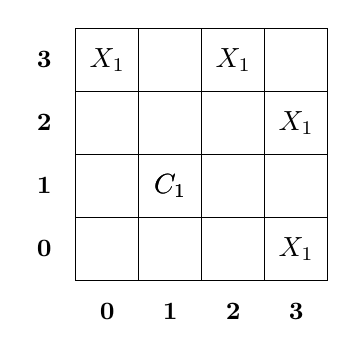
\begin{tikzpicture}[scale=0.8]
        % Dibuja el tablero
        \foreach \x in {0,1,2,3} {
            \foreach \y in {0,1,2,3} {
                \fill[white] (\x,\y) rectangle (\x+1,\y+1);
                \draw (\x,\y) rectangle (\x+1,\y+1);
            }
        }
    
        % Marcar los caballos con C_i
        \node at (1.5, 1.5) {$C_1$}; % (1,1)
    
        % Marcar las casillas alcanzables con X_i
        \node at (0.5, 3.5) {$X_1$}; % (0,3)
        \node at (1.5, 1.5) {$C_1$}; % (1,1)
        \node at (2.5, 3.5) {$X_1$}; % (2,3)
        \node at (3.5, 0.5) {$X_1$}; % (3,0)
        \node at (3.5, 2.5) {$X_1$}; % (3,2)
    
        % Etiquetas
        \foreach \x in {0,...,3} {
            \foreach \y in {0,...,3} {
                % Etiquetas de fila y columna
                \ifnum\x=0
                    \node at (-0.5,\y+0.5) {\textbf{\small \y}};
                \fi
                \ifnum\y=0
                    \node at (\x+0.5,-0.5) {\textbf{\small \x}};
                \fi
            }
        }
    \end{tikzpicture}
    \end{center}
    \item En otro caso se devuelve true pues todas las casillas son alcanzables (algunas por más de un caballo).
    \begin{center}
    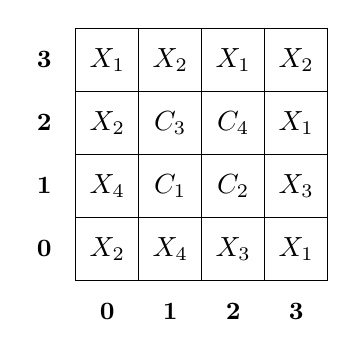
\begin{tikzpicture}[scale=0.8]
        % Dibuja el tablero
        \foreach \x in {0,1,2,3} {
            \foreach \y in {0,1,2,3} {
                \fill[white] (\x,\y) rectangle (\x+1,\y+1);
                \draw (\x,\y) rectangle (\x+1,\y+1);
            }
        }
        
        % Caballos en posiciones C_i
        \node at (1.5, 1.5) {$C_1$}; % (1,1)
        \node at (2.5, 1.5) {$C_2$}; % (2,1)
        \node at (1.5, 2.5) {$C_3$}; % (1,2)
        \node at (2.5, 2.5) {$C_4$}; % (2,2)
    
        % Marcar las casillas alcanzables con X_i
        \node at (0.5, 0.5) {$X_2$}; % (0,0)
        \node at (0.5, 1.5) {$X_4$}; % (0,1)
        \node at (0.5, 2.5) {$X_2$}; % (0,2)
        \node at (0.5, 3.5) {$X_1$}; % (0,3)
        \node at (1.5, 0.5) {$X_4$}; % (1,0)
        \node at (1.5, 3.5) {$X_2$}; % (1,3)
        \node at (2.5, 0.5) {$X_3$}; % (2,0)
        \node at (2.5, 3.5) {$X_1$}; % (2,3)
        \node at (3.5, 0.5) {$X_1$}; % (3,0)
        \node at (3.5, 1.5) {$X_3$}; % (3,1)
        \node at (3.5, 2.5) {$X_1$}; % (3,2)
        \node at (3.5, 3.5) {$X_2$}; % (3,3)
    
        % Etiquetas
        \foreach \x in {0,...,3} {
            \foreach \y in {0,...,3} {
                % Etiquetas de fila y columna
                \ifnum\x=0
                    \node at (-0.5,\y+0.5) {\textbf{\small \y}};
                \fi
                \ifnum\y=0
                    \node at (\x+0.5,-0.5) {\textbf{\small \x}};
                \fi
            }
        }
        
    \end{tikzpicture}
    \end{center}
\end{itemize}

    \item \textbf{Dama amenazada}\\
    Dado un tablero de ajedrez donde se ubican solo damas (reinas), determine si existe alguna que amenace a otra. La representación del tablero será un array bidimensional de bool donde solo habrá true en las casillas donde haya una reina.


    \item \textbf{Validación de un Sudoku}\\
    En este ejercicio, implementarás un programa que valide si un tablero de Sudoku es válido. El programa recibirá como entrada un tablero representado como una matriz de \(9 \times 9\), un tablero de Sudoku debe cumplir con las siguientes reglas:
    \begin{itemize}
        \item Cada fila debe contener los números del \(1\) al \(9\) sin repetir.
        \item Cada columna debe contener los números del \(1\) al \(9\) sin repetir.
        \item Cada subcuadrícula de \(3 \times 3\) debe contener los números del \(1\) al \(9\) sin repetir.
    \end{itemize}

    Algunas celdas estarán vacías, representadas por un \(0\).

    \subsection*{Ejemplo de entrada}
    \[
    \text{sudoku} = 
    \begin{bmatrix}
    5 & 3 & 0 & 0 & 7 & 0 & 0 & 0 & 0 \\
    6 & 0 & 0 & 1 & 9 & 5 & 0 & 0 & 0 \\
    0 & 9 & 8 & 0 & 0 & 0 & 0 & 6 & 0 \\
    8 & 0 & 0 & 0 & 6 & 0 & 0 & 0 & 3 \\
    4 & 0 & 0 & 8 & 0 & 3 & 0 & 0 & 1 \\
    7 & 0 & 0 & 0 & 2 & 0 & 0 & 0 & 6 \\
    0 & 6 & 0 & 0 & 0 & 0 & 2 & 8 & 0 \\
    0 & 0 & 0 & 4 & 1 & 9 & 0 & 0 & 5 \\
    0 & 0 & 0 & 0 & 8 & 0 & 0 & 7 & 9 \\
    \end{bmatrix}
    \]
    \subsection*{Salida esperada}

    \begin{itemize}
        \item Para el tablero de entrada anterior, el programa debe devolver:
        \[
        \text{El tablero de Sudoku es válido: Sí.}
        \]
        \item Si se modifica la celda \((1,2)\) del tablero para que contenga un \(5\), el programa debe devolver:
        \[
        \text{El tablero de Sudoku es válido: No.}
        \]
    \end{itemize}

    \item \textbf{Validación de movimientos en Ajedrez}\\
    Tu misión es implementar un programa que determine si un movimiento de una pieza de ajedrez es válido. Usa el siguiente \textcolor{blue}{enum} para representar las piezas:

    \begin{lstlisting}
    public enum ChessPiece
    {
        None,           // No piece (empty square)
        WhitePawn,
        WhiteKnight,
        WhiteBishop,
        WhiteRook,
        WhiteQueen,
        WhiteKing,
        BlackPawn,
        BlackKnight,
        BlackBishop,
        BlackRook,
        BlackQueen,
        BlackKing
    }
    \end{lstlisting}

    El tablero se representará como una matriz de \(8 \times 8\) de tipo \texttt{ChessPiece}, donde cada celda indica la pieza presente o está vacía (\texttt{None}).

    Tu programa debe recibir como entrada un tablero, junto con las coordenadas iniciales y finales del movimiento, representadas como \((x_1, y_1)\) y \((x_2, y_2)\); a partir de esta información, deberá determinar si el movimiento indicado es válido, considerando las reglas correspondientes a la pieza ubicada en la posición inicial.

    Las reglas de movimiento para cada tipo de pieza son las siguientes:
    \begin{itemize}
        \item \textbf{Peones} (Pawn): Avanzan (o retroceden, si son negros) una casilla hacia adelante, excepto en su primer movimiento, donde pueden avanzar dos casillas. Capturan piezas únicamente en diagonal y no pueden avanzar hacia casillas ocupadas.
        \item \textbf{Caballos} (Knight): Se mueven en forma de "L", moviéndose dos casillas en una dirección y una en perpendicular. Pueden saltar sobre otras piezas, pero solo ocupan la casilla de destino si está vacía o contiene una pieza del oponente.
        \item \textbf{Alfiles} (Bishop): Se mueven únicamente en diagonal, cualquier cantidad de casillas. No pueden atravesar ni ocupar casillas ocupadas, salvo para capturar una pieza del oponente en la casilla de destino.
        \item \textbf{Torres} (Rook): Se mueven en línea recta, ya sea horizontal o verticalmente, cualquier número de casillas. No pueden atravesar ni ocupar casillas ocupadas, salvo para capturar una pieza del oponente en la casilla de destino.
        \item \textbf{Reinas} (Queen): Combinan los movimientos de las torres y los alfiles, moviéndose tanto en línea recta como en diagonal.
        \item \textbf{Reyes} (King): Se mueven una casilla en cualquier dirección: horizontal, vertical o diagonal. No pueden moverse a una casilla ocupada salvo para capturar una pieza del oponente en la casilla de destino.
    \end{itemize}
    
    \textbf{Nota}: El ejercicio no requiere implementar lógica adicional como detectar jaque, jaque mate, enroque o promoción de peones. Solo se debe comprobar si el movimiento en cuestión cumple con las reglas básicas de la pieza.

    \item \textbf{Jaque al rey}\\
    Implemente un método que reciba un tablero de ajedrez, y determine si el rey negro está amenazado por alguna pieza blanca. 

El método deberá tener la siguiente signatura:

\begin{lstlisting}
    public enum ChessPiece
    {
        None,           // No piece (empty square)
        WhitePawn,
        WhiteKnight,
        WhiteBishop,
        WhiteRook,
        WhiteQueen,
        WhiteKing,
        BlackPawn,
        BlackKnight,
        BlackBishop,
        BlackRook,
        BlackQueen,
        BlackKing
    }
    
    public static bool IsBlackKingInCheck(ChessPiece[,] board)
    {
        // ...
    }
\end{lstlisting}


    \item \textbf{El Mago y el Bosque Encantado}\\
    En un bosque encantado, un mago ha decidido medir el poder de su hechizo de teletransportación. El bosque está representado como una cuadrícula de \(N \times M\), donde cada celda puede estar despejada o bloqueada por un obstáculo mágico. El mago comienza en una posición definida por el usuario, y desea calcular cuán lejos puede llegar su hechizo desde esa posición, sin atravesar los obstáculos.
    \begin{itemize}
        \item El bosque se representa como una matriz booleana: 
        \begin{itemize}
            \item \texttt{false}: La celda está despejada (el hechizo puede pasar).  
            \item \texttt{true}: La celda está bloqueada (el hechizo no puede pasar).  
        \end{itemize}
        \item La entrada incluye la posición inicial del mago \((x, y)\).  
        \item El resultado debe ser una matriz que indique la distancia desde la posición inicial hasta cada celda accesible, respetando los obstáculos. Las celdas bloqueadas deben marcarse como \(-1\) en la salida.  
    \end{itemize}

    \subsection*{Ejemplo}
    \text{Entrada:}
    \begin{itemize}
            \item Posición inicial del mago: \((2, 2)\).  
            \item Bosque: 
            \[ 
            \begin{bmatrix}
                \texttt{false} & \texttt{false} & \texttt{false} & \texttt{false} & \texttt{false} \\
                \texttt{false} & \texttt{false} & \texttt{false} & \texttt{true}  & \texttt{false} \\
                \texttt{false} & \texttt{false} & \texttt{false} & \texttt{false} & \texttt{false} \\
                \texttt{false} & \texttt{false} & \texttt{false} & \texttt{true}  & \texttt{false} \\
                \texttt{false} & \texttt{false} & \texttt{false} & \texttt{false} & \texttt{false} \\
                \end{bmatrix}
            \]
    \end{itemize}
    \text{Salida:}
    \[
    \begin{bmatrix}
    4 & 3 & 2 & 3 & 4 \\
    3 & 2 & 1 & -1 & 3 \\
    2 & 1 & 0 & 1  & 2 \\
    3 & 2 & 1 & -1 & 3 \\
    4 & 3 & 2 & 3  & 4 \\
    \end{bmatrix}
    \]

    \item \textbf{Recorriendo islas}\\
    El mapa de unas islas está modelado mediante un array bidimensional booleano, donde las casillas con valor true son secciones de tierra firme y las casillas con valor false son agua. Se desea encontrar cuál es la distancia mínima a recorrer entre el par de casillas \( (f_i, c_i) \) y \( (f_s, c_s) \) si solo se puede transitar por secciones de tierra firme.

\end{enumerate}
